


\startp
\upar{Оптимизация отстройки лучей МОЛ}
Для оптимизации количества атомов тулия в МОЛ была измерена зависимость $N(t, \delta)$ и определен её оптимум. Величина отстройки $\delta$ луча МОЛ контролировалась с помощью напряжения, подаваемого на АОМ. В соответсвии с процедурой, описанной в разделе \ref{subsec:Обработка фотографии}, измерялось полное число атомов $N$ в ловушке в различные моменты времени $t$, для раличной отстройки $\delta$. 

Полученные данные (рис. \ref{fig:motload}a) аппроксимировались зависимостью, вида
\begin{equation}
	F(t) = \sub{N}{max} \left(1- e^{-\sub{t}{load}/\tau}\right),
\end{equation}
где $\tau$ -- характерное время загрузки, $\sub{N}{max}$ -- предельное число атомов. Из \eqref{eq:Ntd} видно, что $\sub{N}{max} = \sqrt{\sub{\Phi}{load}/\beta}$, $\tau = 1/\sqrt{\beta \sub{\Phi}{load}}$.

\begin{figure}[ht]
    \centering
    \subfigure[]{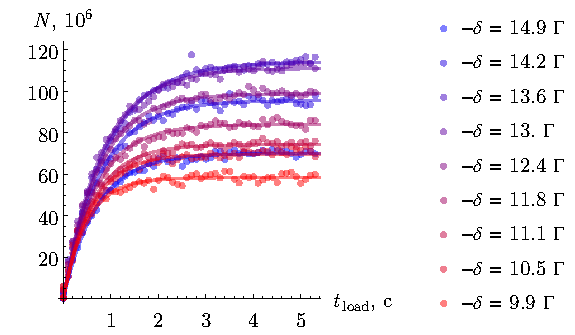
\includegraphics{figs/motload_v2.pdf}}
    \hspace{10 mm} 
    \subfigure[]{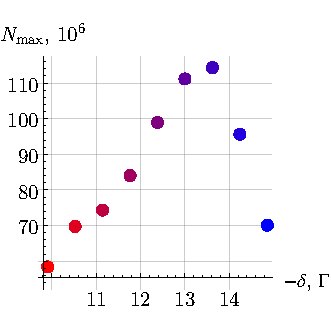
\includegraphics{figs/motload2_v2.pdf}}
    \caption{a) Динамика загрузки МОЛ для различных значений отстройки б)  Зависимость максимального числа атомов в МОЛ от величины отстройки $\delta$}
    \label{fig:motload}
\end{figure}




По зависимости $\sub{N}{max} (\delta \nu)$ (рис. \ref{fig:motload}b) было определено оптимальное значене отстройки $\delta$ лазерного луча МОЛ: максимальное значение атомов в ловушке $\sub{N}{max}$ составило $114 \times 10^6$ атомов. 
Наблюдаемое значение $\sub{\Phi}{load} = \sub{N}{max} / \tau \sim  10^{8}\,\text{c}^{-1}$.


% \unewpage


\upar{Оптимизация токов ЗЗ} Магнитное поле в ЗЗ контролируется с помощью токов, подаваемых на большую и маленькую катушку (рис. \ref{fig:zB}). Аналогично оптимизации отстройки лучей МОЛ на времени загрузки 5\,с измерялось количество атомов в МОЛ $N$ для различных значений тока маленькой катушки $\sub{I}{small}$ и большой катушки $\sub{I}{big}$ (рис. \ref{fig:IZ1}). Оптимум находится в районе $\sub{I}{big} = 35\,$А  и $\sub{I}{small}=18\,$А.

% отстройка патоки
\begin{figure}[ht]
    \centering
    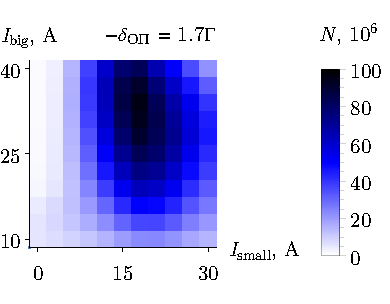
\includegraphics{figs/IZ1.pdf}
    \caption{Зависимость количества загруженных за 5с в МОЛ атомов от величины токов малой и большой катушки ЗЗ. Зависимость снята  при оптимальной отстройке лучей ОП $\subt{\delta}{ОП}$.}
    \label{fig:IZ1}
\end{figure}

Аналогичные измерения проделаны для других отсроек лучей ОП (рис. \ref{fig:IZ2}), определено, что исходное значение $\subt{\delta}{ОП} = 9.4 \Gamma$ является локально оптимальным.

\begin{figure}[ht]
    \centering
    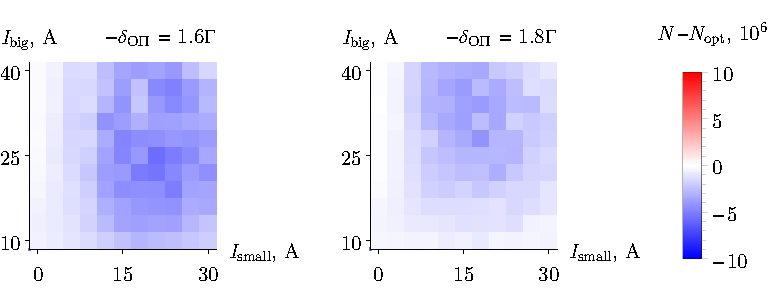
\includegraphics{figs/IZ2.pdf}
    \caption{Зависимость количества загруженных за 5с при оптимальной отстройке лучей ОП в МОЛ атомов от величины токов малой и большой катушки ЗЗ. Зависимость снята при $\subt{\delta}{ОП}$ большей и меньшей оптимального значения в $\subt{\delta}{ОП} = 9.4 \Gamma$.}
    \label{fig:IZ2}
\end{figure}